% !Mode:: "TeX:UTF-8"
%% 请使用 XeLaTeX 编译本文.制作者:中南大学,电气1705陈宝轩,2020.1.16
% \documentclass{WHUBachelor}% 选项 forprint: 交付打印时添加, 避免彩色链接字迹打印偏淡. 即使用下一行:
\documentclass[forprint]{CSUBachelor}
\usepackage{listings}				%对代码进行抄录环境的宏包
\usepackage{setspace}				%行间距
\usepackage{float}
\usepackage{enumerate}		%公式
\usepackage{amsmath}
\usepackage{changepage}		%段落缩进用的

\begin{document}

\title{PCB电磁兼容设计}
\Etitle{PCB electromagnetic compatibility design} % 英文题目
\author{陈宝轩}                            		% 作者名字
\Eauthor{CHEN Baoxuan}           		 % 作者英文名A
\Csupervisor{啦啦啦\quad 教授}       	 % 指导教师中文名、职称
\Esupervisor{Prof.cc}    				 % 指导教师英文名、职称
\Cmajor{电气工程及其自动化}                 	 % 专业中文名
\Emajor{Electrical Engineering and Automation} % 专业英文名
\Cschoolname{自动化学院}         		 % 学院名
\Eschoolname{School of Automation} 		 % 学院英文名.
\Cclassname{电气1705班}      			 % 专业班级中文名

\date{2020年6月}                    		% 日期, 要注意和英文日期一致!!
\Edate{June, 2020}                      	% 英文封面日期

%-----------------------------------------------------------------------------
\pdfbookmark[0]{封面}{title}         % 封面页加到 pdf 书签
\maketitle
\frontmatter
\pagenumbering{Roman}              % 正文之前的页码用大写罗马字母编号.
%-----------------------------------------------------------------------------
% !Mode:: "TeX:UTF-8"

%自行填写: (1) 中文摘要及关键词 (2) 英文摘要及关键词

%------------------------------------------中文摘要----------------------------------------------------
\begin{cnabstract}

本文在武汉大学模板的基础上,主要介绍和讨论了中南大学本科毕业论文的~\LaTeX~模板.

指明了编译方法,讨论了一些\LaTeX{}的使用小技巧
\end{cnabstract}
\par
\vspace*{1em}	%空一行,再写关键词

%-------------------------------------- 关键词 ---------------------------------------------------
%注意: 每个关键词之间空一格汉字的长度,最后一个关键词后无标点符号
\cnkeywords{\LaTeX{} \phantom{哈}中南大学\phantom{哈}模板\phantom{哈}陈宝轩想睡觉}

%------------------------------英文摘要---------------------------------------

\begin{enabstract}
This thesis is a study on the theory of \dots.

\end{enabstract}
\par
\vspace*{2em}

%------------------------------- Key words ---------------------------------------
%%%%-- 注意: 每个关键词之间空两个英文字母的长度,最后一个关键词后无标点符号
 \enkeywords{\LaTeX{}\phantom{cc}CSU\phantom{cc}template\phantom{cc}sleepy}
    % 加入摘要
%-------------------------------把目录加入到书签---------------------------------%
\iffalse	% 注释
\pdfbookmark[0]{目录}{toc}
\tableofcontents   %显示目录
\fi

\mainmatter

%----------------------------------------------正文-------------------------------------%
\chapter{绪论}

\section{aaa}

\subsection{2222}

aaaa ll啦啦啦啦啦


%------------------------------------------ 结束语 -----------------------------------------
% !Mode:: "TeX:UTF-8"
%-----------------------------结束语(或致谢)---------------------------------

\acknowledgement
\addcontentsline{toc}{chapter}{结束语(或致谢)}

(结束语或致谢内容)











 		%致谢

%----------------------------------------- 参考文献-----------------------------------------
\cleardoublepage\phantomsection
\addcontentsline{toc}{chapter}{参考文献}
\wuhao\kaishu
\begin{thebibliography}{00}

  \bibitem{r1} 阮毅,陈伯时. 电气拖动自动化控制系统. 第三版.北京:机械工业出版社, 2018:11

  \bibitem{r2} 天津电气传动设计研究所. 电气传动自动化技术手册.第三版.北京:机械工业 出版社,2016:11
  
\end{thebibliography}

%----------------------------------- 附录-----------------------------------
\appendix

\chapter{公式、图片、表格等}

公式:\ref{con:1}

	\vspace{-2em}		% 公式与文字距离近一点
	\begin{center}
	\begin{gather}		% gather可以多行公式,equation就不可以
		%\nonumber		% 不要序号显示
		%\begin{cases}	% 大括号
		R_n=K_nR_0=23.8307\times40=953.228K\Omega\\
		C_n=\frac{\tau_n}{R_n}=\frac{0.087}{100\times 10^3}F=0.087\mu F\\
		C_{on}=\frac{4T_{on}}{R_o}=\frac{40\times 0.01}{40000}F=1\mu F
		%\end{cases}
	\label{con:1}
	\end{gather}
	\end{center}

图片:\ref{fig:left_v}

\begin{figure}[H]
\centering
\setlength{\abovecaptionskip}{2pt}\setlength{\belowcaptionskip}{10pt}
  %\includegraphics[width=15cm, height=10cm]{fengji.jpg}
	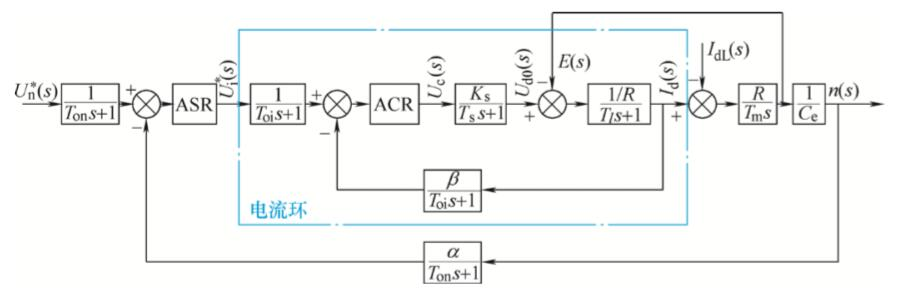
\includegraphics[scale=0.6]{6-2.jpg}
  \caption{\heiti\zihao{5}系统动态结构图}
  \label{fig:6-2}
\end{figure}

\begin{figure}[H]
\centering
\setlength{\abovecaptionskip}{2pt}\setlength{\belowcaptionskip}{10pt}	
%将图片标题紧靠图片		这个管用,表格的不管用
  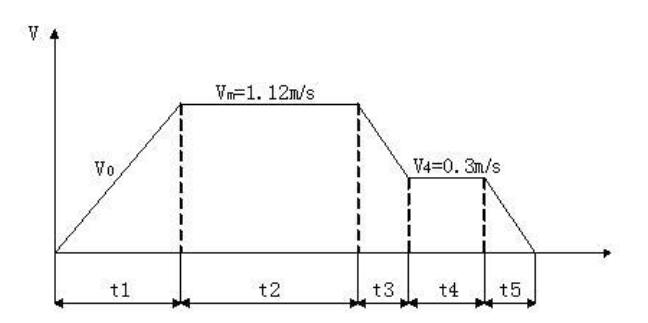
\includegraphics[width=\textwidth]{left_v.jpg}
  \caption{\heiti\zihao{5}提升机提升速度图}
  \label{fig:left_v}
\end{figure}

表格:\ref{11}

\begin{table}[h]
  \centering
  \caption{集中整流线路变压器电压计算系数(电感性负载)}
	\renewcommand\arraystretch{1.5}	%行间距1.5倍
  \begin{tabular}{*{4}c}
     \hline
     % after \\: \hline or \cline{col1-col2} \cline{col3-col4} ...
     电路类型 & A  & 电路类型  & A \\
	\hline
     单相半波 & \quad 0.45 \quad & 三相半波  & \quad 1.17 \quad \\
     单相桥式 & \quad 0.90 \quad & 三相桥式  & \quad 2.34 \quad \\
     \hline
   \end{tabular}
	\label{11}
\end{table}

项目清单:

\begin{itemize}
    \item 图中$W_n(s)$为速度调节器的传递函数;
	\item $W_i(s)$为电流调节器的传递函数;
	\item $T_s$为晶闸管平均失控时间常数,对于三相桥式整流电路,取$T_s= 0.00167s$;
	\item $T_M$为电动机机电时间常数,取$T_M=0.1s$;
	\item $T_i$为电动机电磁时间常数,$T_i=LR=0.005\times0.18=0.0277s$;
	\item $T_m$为机电时间常数,计算得$T_m=0.01s$;
	\item $C_e$为电动机转矩系数,由上面知可取$0.56436V/(r/min)$;
	\item $T_{oi}$为电流反馈滤波时间,取$T_{oi}=0.002s$;
	\item $T_{on}$为速度反馈滤波时间,取$T_{on}=0.01s$;
\end{itemize}


序号:

\begin{enumerate}[\phantom{哈哈}(1)]
		
	{\bf \item 匀速阶段\quad $t_1\sim t_2$}

\begin{adjustwidth}{-2em}{0em}
\hspace{2em}直流电机提升时,$T=0$,匀速上升。

下放时,也有$T=0$,采用能耗制动、闭环控制,单闭环速度控制系统由与距离有关的理想速度给定电路、速度负反馈电路、PID调节器、移相触发电路及双向可控硅能耗制动电路组成,下放速度由PID调节。

	\begin{center}
	\begin{gather}
		\begin{cases}
		T_e>0\\
		T_L<0\\
		T=T_e+T_L=0
		\end{cases}
	\end{gather}
	\end{center}

\end{adjustwidth}

	{\bf \item 主减速阶段\quad $t_2\sim t_3$}
	{\bf \item 爬升阶段\quad $t_3\sim t_4$}

\end{enumerate}

\iffalse	% 注释
% 这里面的不知为啥报错,不管了
\begin{enumerate}[itemsep=0pt,parsep=0pt,label=(\arabic*)]
	\item  速度闭环控制、电流闭环控制、力矩控制、弱磁控制;
	\item  S 形上升曲线(减少提升机钢丝绳抖动);
	\item  全数字控制自诊断和故障显示(PLC+触摸屏);
\end{enumerate}
\fi 


\chapter{PLC通信程序设计}

PLC 作为控制系统中的下位机,不主动发送数据而是被动的响应上位机的命令,根据上位机的指令进行数据发送和接收。因为本学期正好学习了《电气控制 与 PLC 应用技术》课程,因此试着完成了通信程序的设计:PLC 的通信程序由主程序、三个子程序和三个中断组成。 

PLC 在第一次扫描时开始执行初始化子程序,对端口及 RCV 指令初始化。初始化后,就使端口处于接受状态。RCV 指令将接收到的数据保存到接收缓冲区,同时产生接受完成中断。PLC 每接到一条指令后都发送一条反馈信息,完成发送后产生发送完成中断。梯形图和语句表如下:

\section{第一部分代码}

%设置·为转义字符,这样才可以显示汉语
\lstset{columns=flexable,numbers=left,numberstyle=\footnotesize,escapechar=`,xleftmargin=2em,xrightmargin=2em, aboveskip=0em}

\begin{spacing}{1}
\begin{lstlisting}[language=C]
/*hello.c*/
#include "sys.h"
int main(void)
{ 
  /*only can use english description*/
	while(1)
	{
	GPIO_ResetBits(GPIOF,GPIO_Pin_9); //`io口初始化`
	GPIO_SetBits(GPIOF,GPIO_Pin_10); 
	delay_ms(500); 
	GPIO_SetBits(GPIOF,GPIO_Pin_9);
	GPIO_ResetBits(GPIOF,GPIO_Pin_10);
	delay_ms(500); 		//`延时$500ms$`,此处可以输入公式
	}	  
}
\end{lstlisting}
\end{spacing}

\cleardoublepage	%目录后的内容从奇数页开始
\end{document}



